\chapter{The tW Channel}
\label{chp:tw}

For the first part of this chapter the decay of the top-quark is discussed. Then the production channels of the top-quark are diagrammed. Finally the production channel of interest and its final state are explained in the context of its background at the Large Hadron Collider (LHC). For more information about the LHC see chapter~\ref{lhc_atlas}.
The diagrams shown in this chapter were created using the code available at~\cite{feyn_repo}.

\section{Top-quark decay}


\section{Top-quark production}

Most commonly top-quarks are created via the strong force in a top- anti-top-quark final state. Both gluon-gluon fusion and \Pquark\APquark-annihilation are possible production processes are possible. Figure~\ref{fig:ttpairLO} shows the processes at leading order (LO). Leading order means that no corrections for additional gluon emission and virtual corrections were taken into account.

\begin{figure}[htbp]
  \begin{subfigure}[b]{0.3\textwidth}
  	\centering
    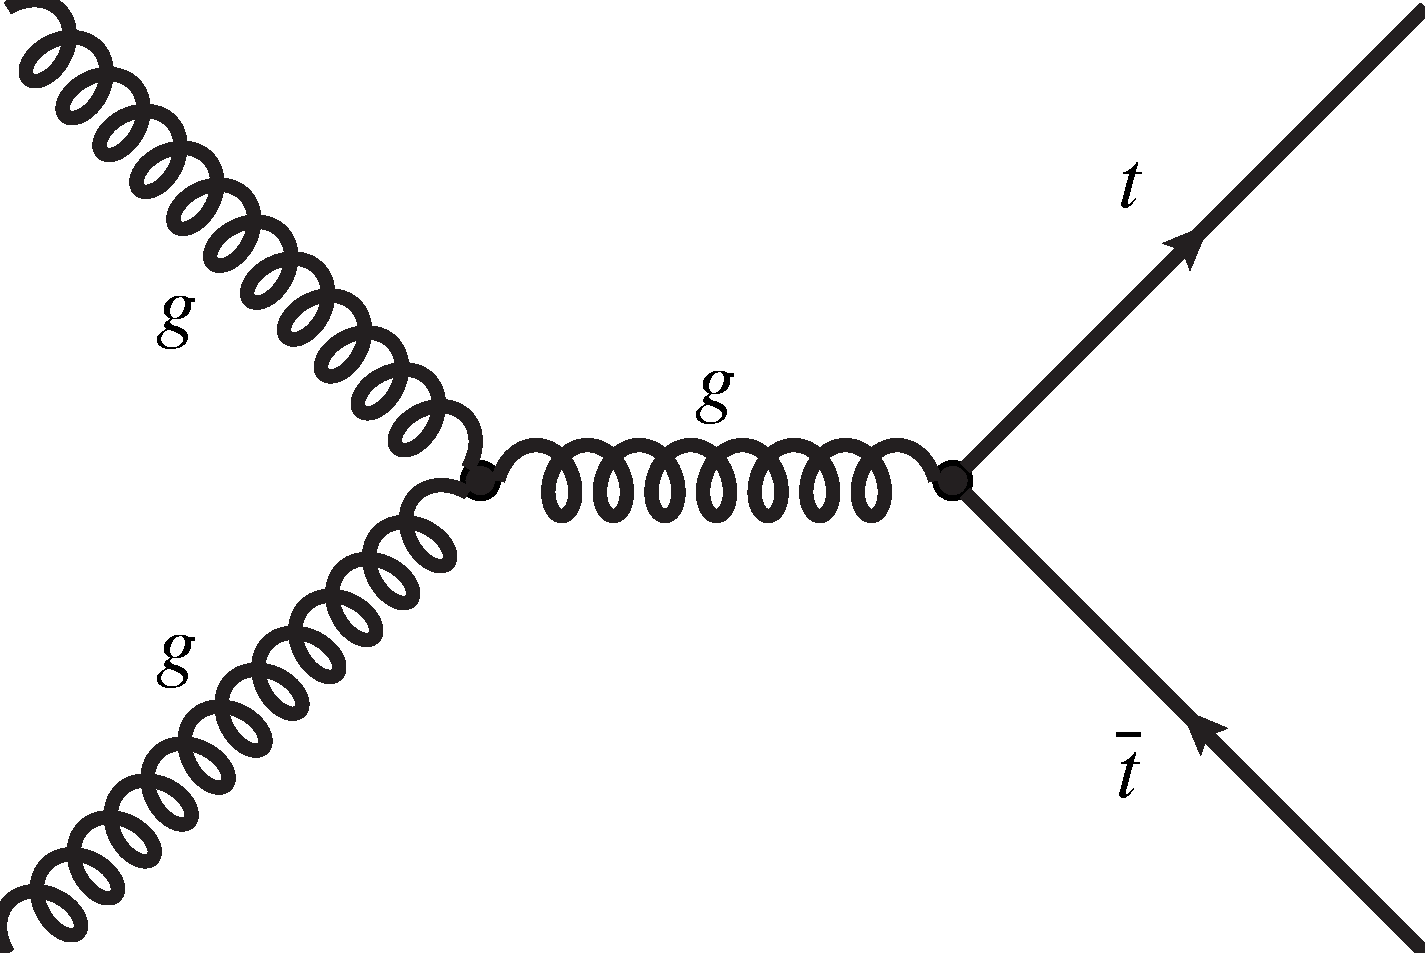
\includegraphics[height=3.5cm]{ttbar_ttbar_1-BW}
%    \caption{Picture 1}
%    \label{fig:1}
  \end{subfigure}
  \quad
  \begin{subfigure}[b]{0.3\textwidth}
  	\centering
    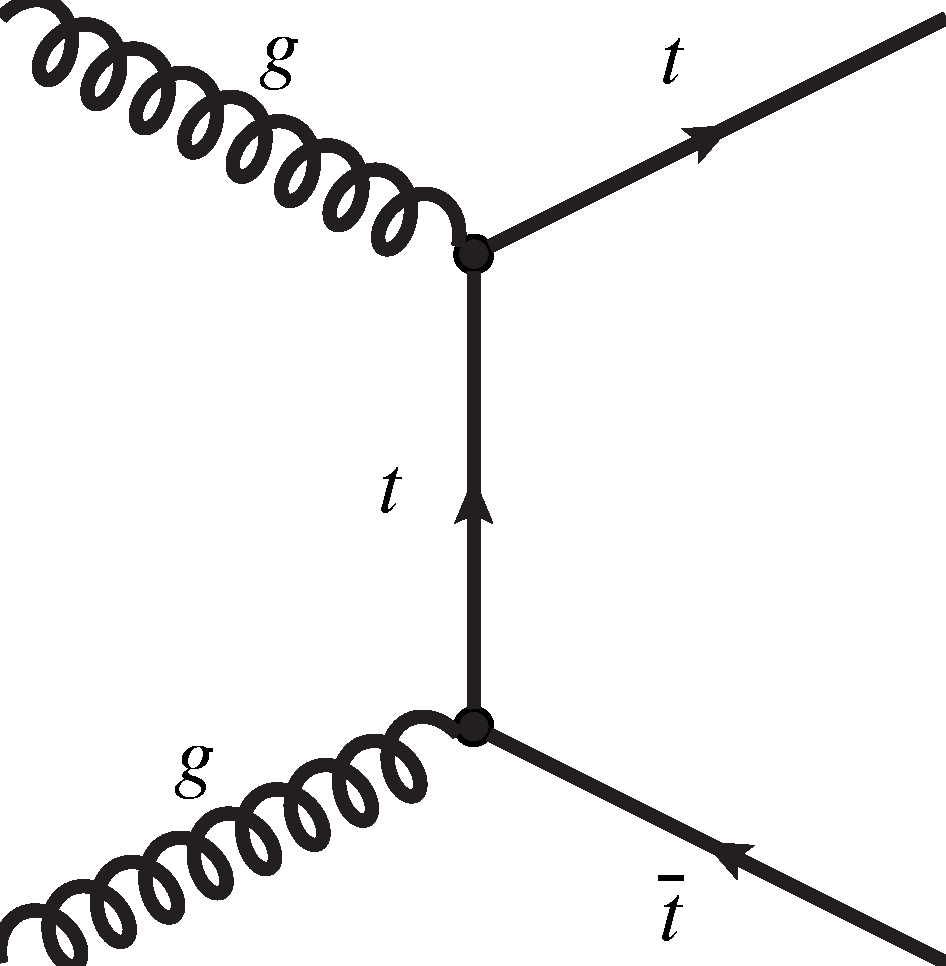
\includegraphics[height=3.5cm]{ttbar_ttbar_2-BW}
%    \caption{Picture 2}
%    \label{fig:2}
  \end{subfigure}
  \quad
  \begin{subfigure}[b]{0.3\textwidth}
  	\centering
    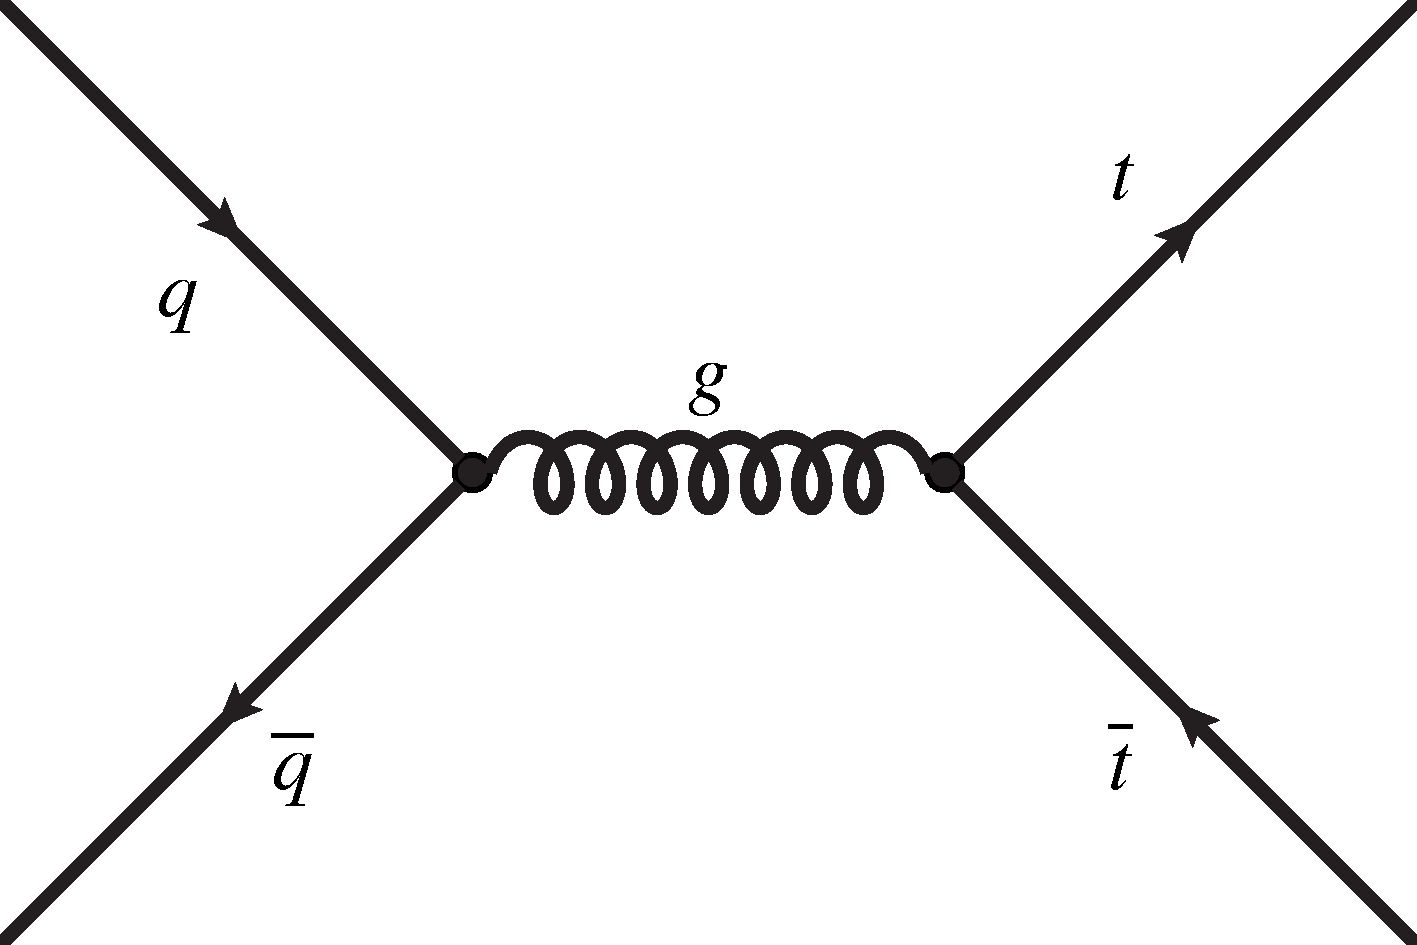
\includegraphics[height=3.5cm]{ttbar_ttbar_3-BW}
%    \caption{Picture 2}
%    \label{fig:2}
  \end{subfigure} 
  \caption[\ttbar pair production feynman diagrams at LO]{\ttbar pair production feynman diagrams at LO.}
  \label{fig:ttpairLO}
\end{figure}

Additionally, top-quarks can be produced as single top-quarks via the electroweak interaction. The dominant process is the production through the interaction of a bottom-quark and a \PW-boson shown in figure~\ref{fig:singletop:virtualWt}. Also possible but the least common is the s-channel involving a virtual \PW-boson displayed in figure~\ref{fig:singletop:virtualWs}. Finally the channel of interest for this work is the \tW-channel diagrammed in figure~\ref{fig:singletop:tW}.

Figure~\ref{fig:tw-decay} shows the final state of the \tW decay with both \PW-bosons decaying leptonically at LO. Therefore the channel is named dilepton channel.
At Next-To-Leading Order (NLO) a gluon splitting can result into a further bottom-quark in the final state. Figure~\ref{fig:nlo} shows the \ttbar final state in comparison to the NLO final state of the \tW-channel. In the final state these channels these channels are not distinguishable, {i.e.}, they interfere. These diagrams will be referred to as doubly resonant, in contrast to the singly resonant diagrams such as diagrammed in figure~\ref{fig:ttpairLO}.
Given that the \ttbar-cross-section is \num{10} orders larger than the \tW-cross-section this gives rise to a NLO correction exceeding the actual LO cross-section. This results in the \tW-channel not being well-defined at NLO.
To allow treating \tW as a separate process a workaround has to be used. There are two possible schemes for handling the interference in the calculation of the cross-section:

\begin{description}
\item[Diagram Removal (DR)] removes all diagrams containing a second top-quark propagator that can be on-shell. It is used for the production of the nominal sample in this work.
\item[Diagram Subtration (DS)] only the \ttbar contribution is cancelled when the top-quark is on-shell. This scheme is used for the systematics sample.
\end{description}

For more information on the schemes and their motivation see section~\ref{sec:systmc},

\begin{figure}[htbp]
  \begin{subfigure}[b]{0.3\textwidth}
  	\centering
    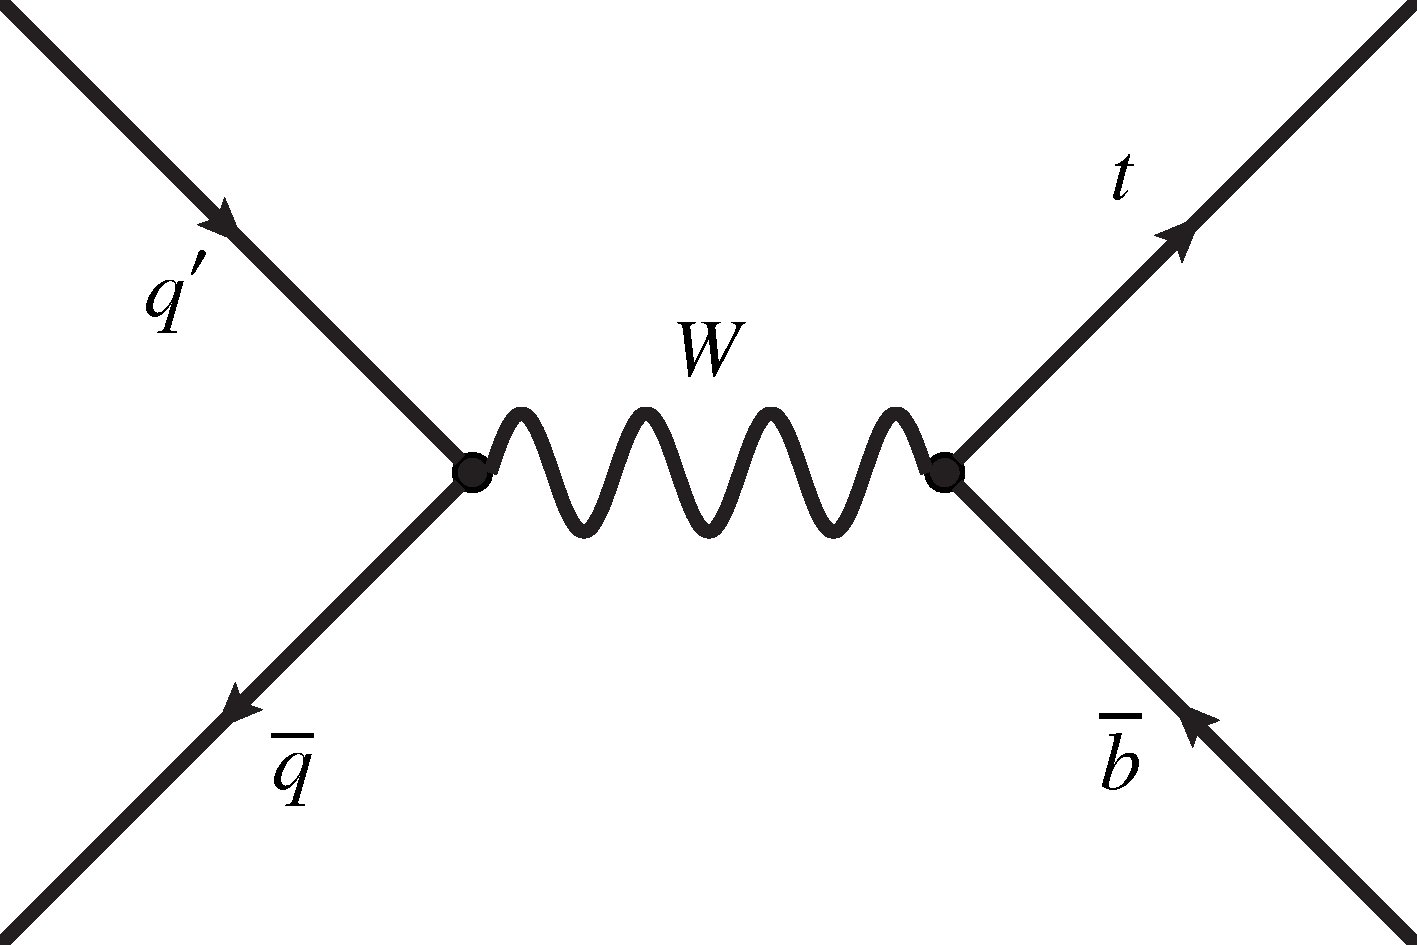
\includegraphics[height=3.5cm]{s-channel}
    \caption{}
    \label{fig:singletop:virtualWt}
  \end{subfigure}
  \quad
  \begin{subfigure}[b]{0.3\textwidth}
  	\centering
    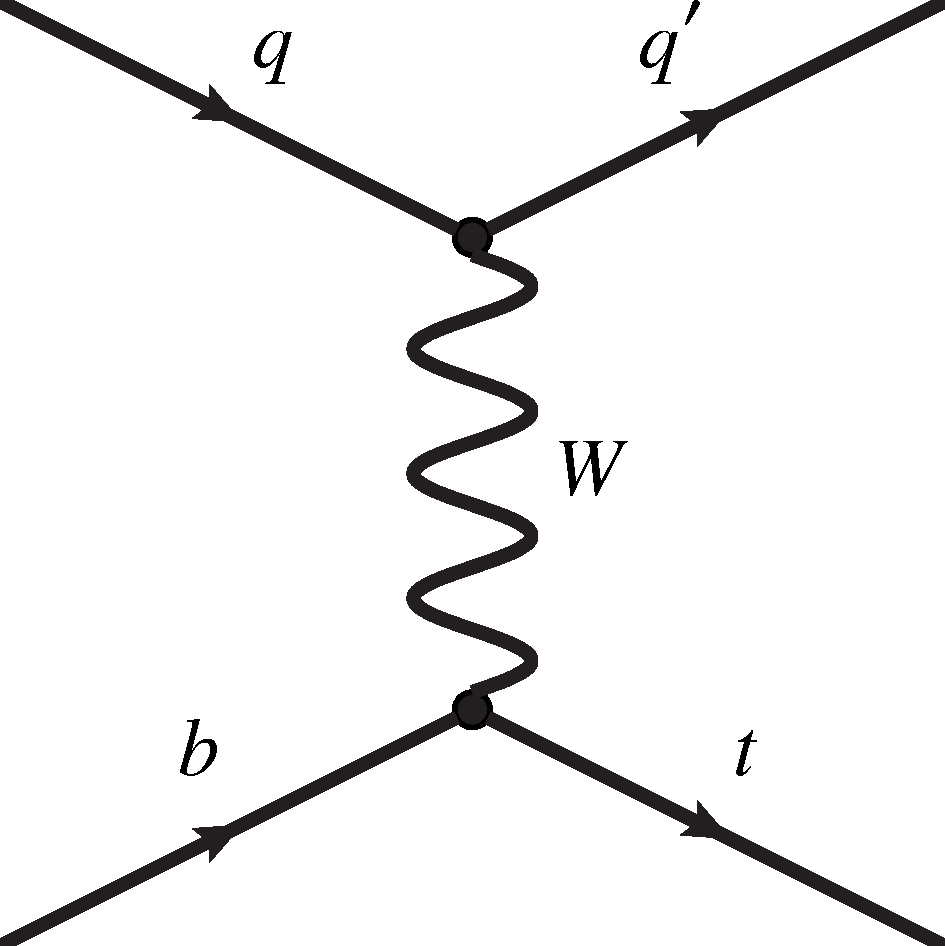
\includegraphics[height=3.5cm]{t-channel}
    \caption{}
    \label{fig:singletop:virtualWs}
  \end{subfigure}
  \quad
  \begin{subfigure}[b]{0.3\textwidth}
  	\centering
    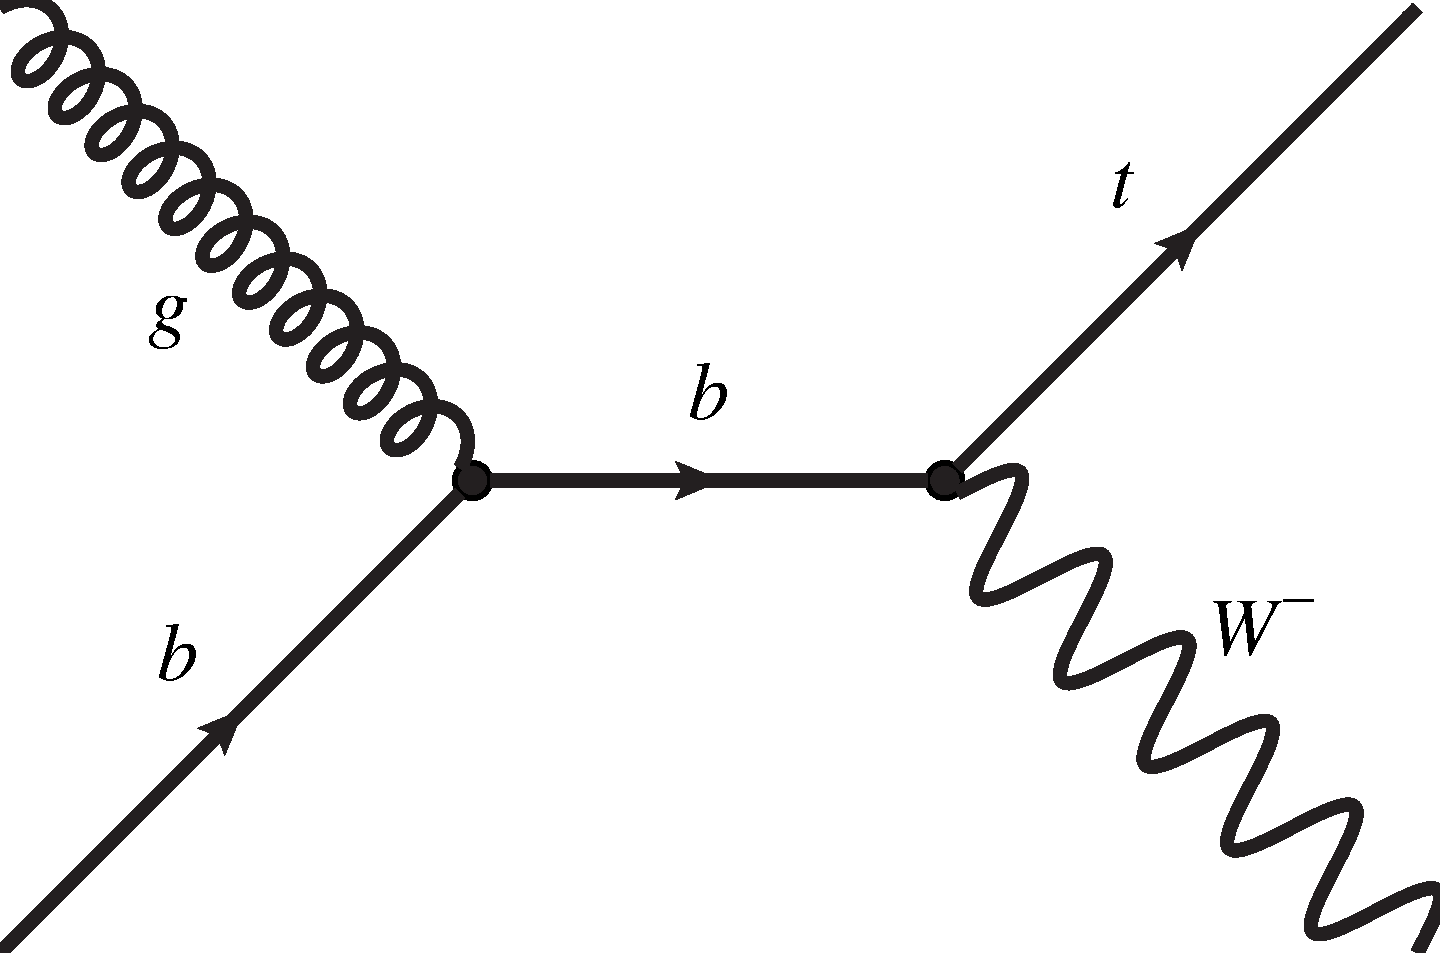
\includegraphics[height=3.5cm]{tW_channel}
    \caption{Picture 2}
	\label{fig:singletop:tW}
  \end{subfigure} 
  \caption[Single-top-production diagrams]{Single-top-production diagrams: s-channel~\subref{fig:singletop:virtualWs}, t-channel~\subref{fig:singletop:virtualWt}, \tW-channel~\subref{fig:singletop:tW}}
  \label{fig:singletop}
\end{figure}


\begin{figure}[htbp]
	\centering
	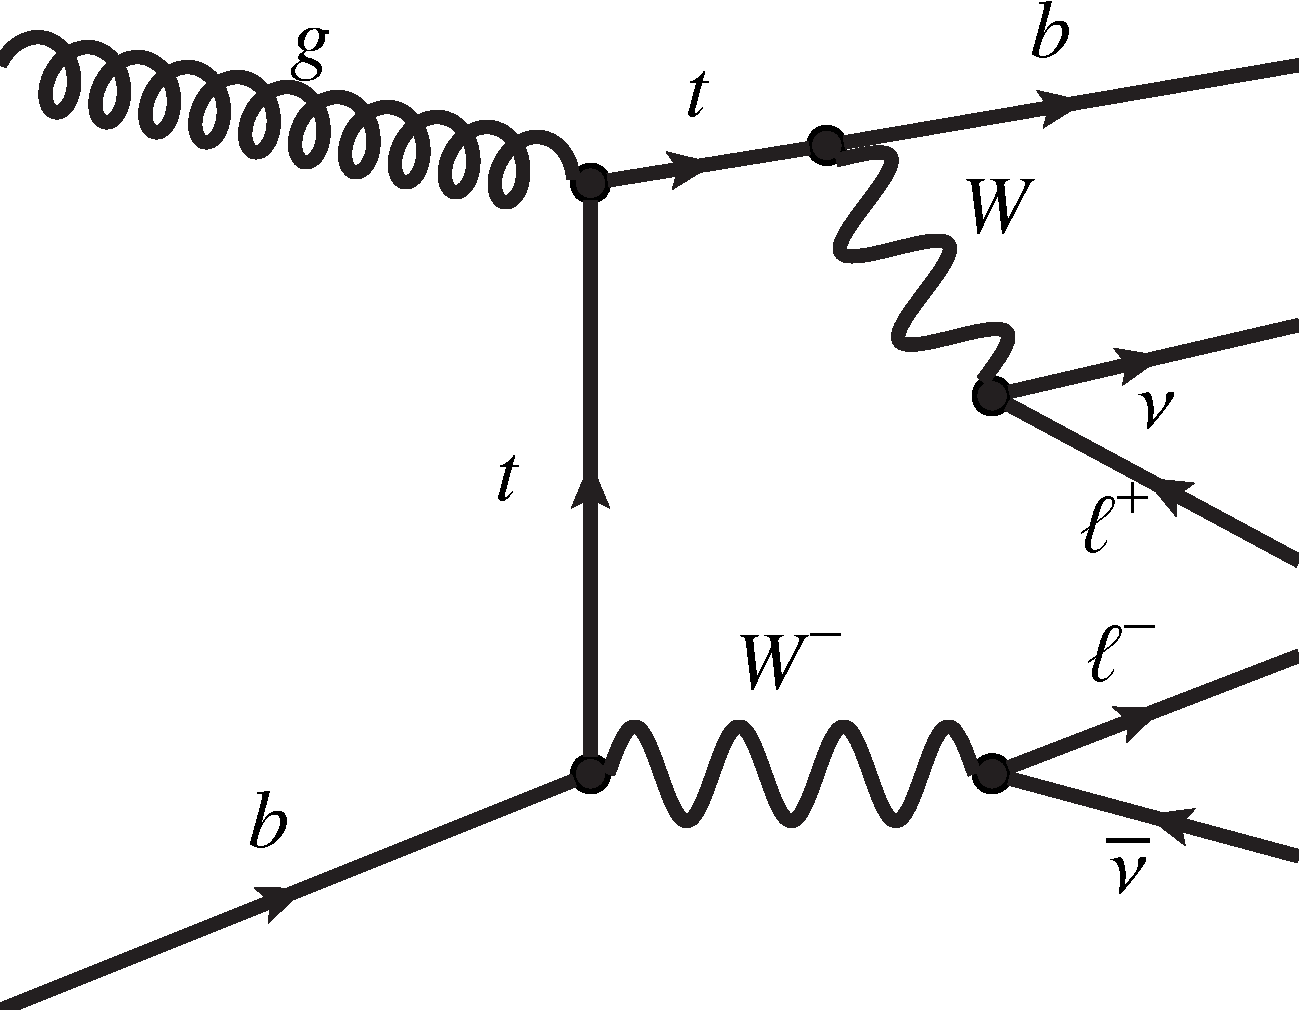
\includegraphics[width=0.8\textwidth]{tW-decay}
	\caption[Final state of a \tW decay]{Final state of a \tW decay. Both \PW-bosons decay leptonically.}
	\label{fig:tw-decay}
\end{figure}

\begin{figure}[htbp]
    \centering
    \begin{subfigure}[b]{0.44\textwidth}
        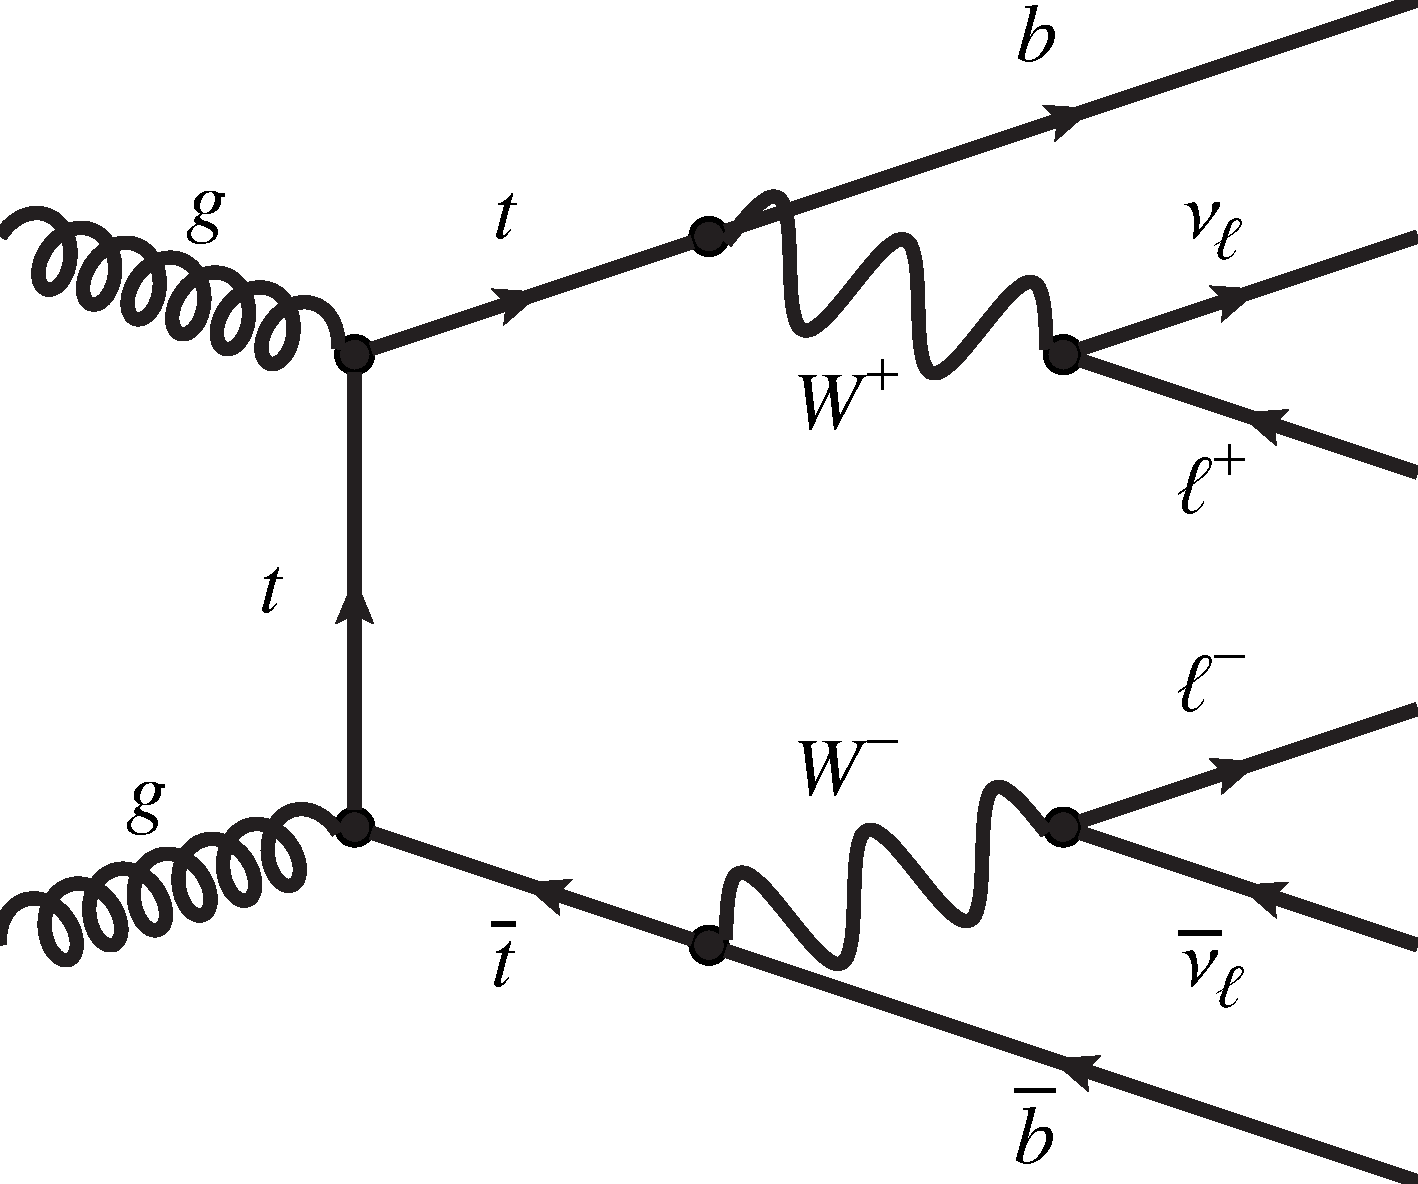
\includegraphics[width=\textwidth]{ttbar-decay}
        \caption{}
        \label{fig:nlo:ttbar}
    \end{subfigure}
\quad
    \begin{subfigure}[b]{0.44\textwidth}
        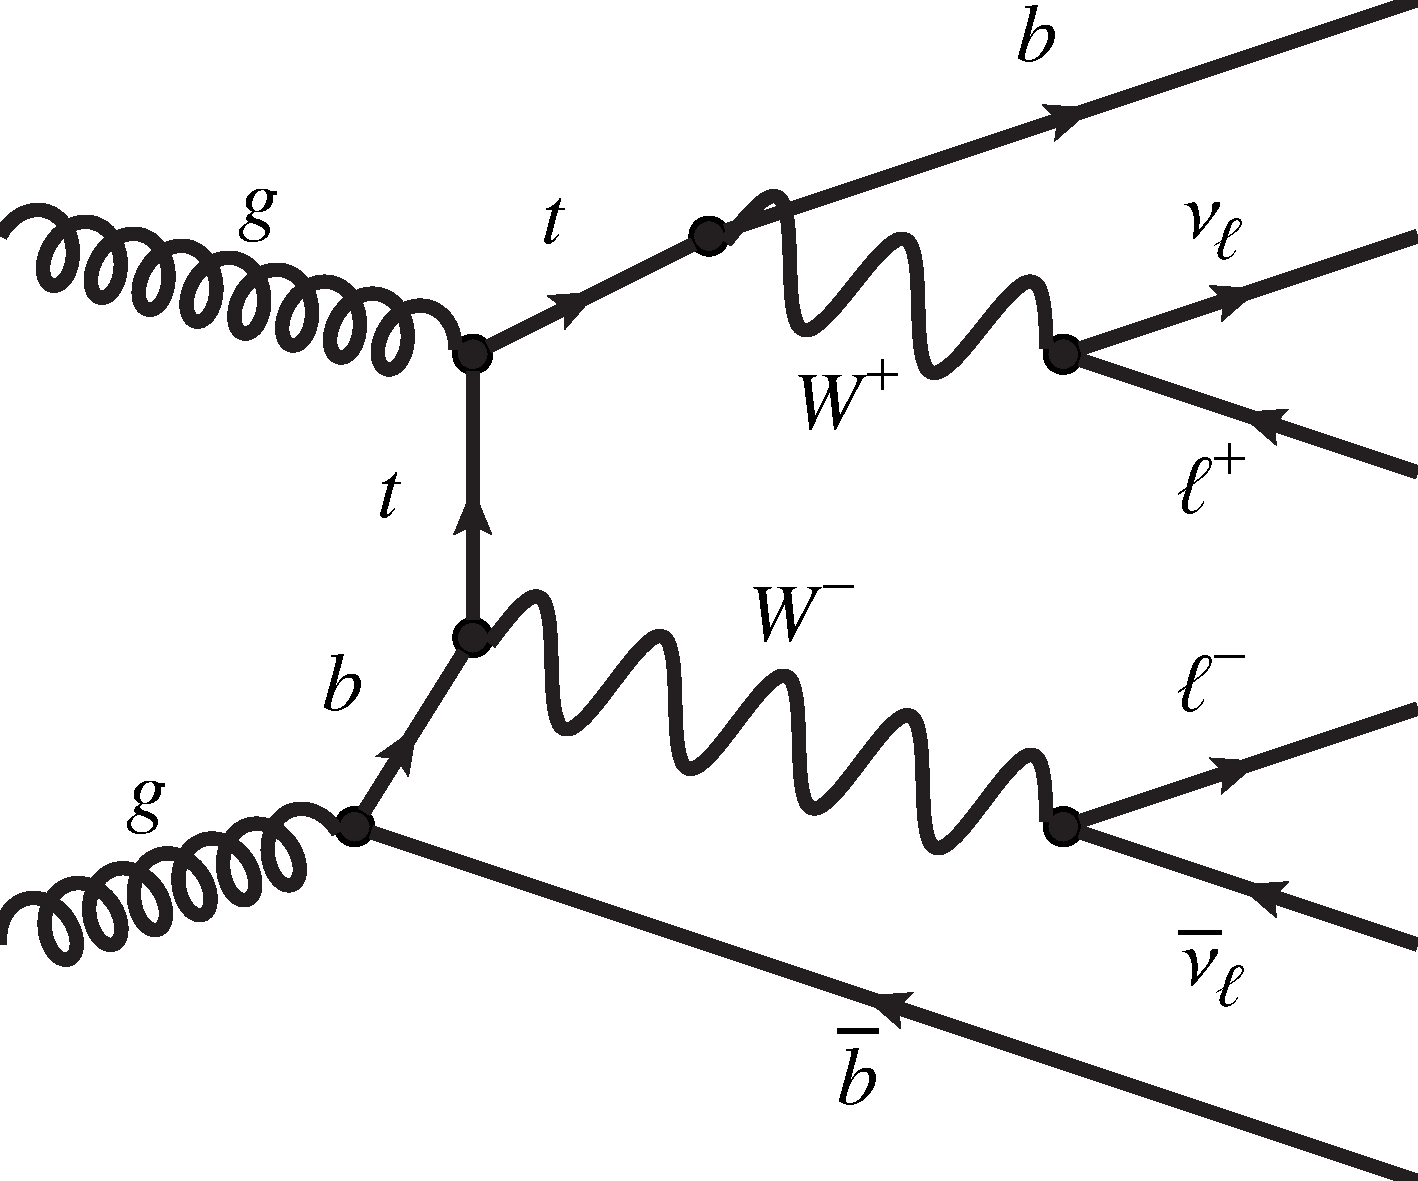
\includegraphics[width=\textwidth]{tw-NLO}
        \caption{}
        \label{fig:nlo:tw}
    \end{subfigure}
    \caption[Comparison of the final state of a \ttbar and \tW event]{Comparison of the final state of a \ttbar event\ref{fig:nlo:ttbar} and a NLO \tW event\ref{fig:nlo:tw}. Both \PW-bosons decay leptonically and the final states are identical.}
	\label{fig:nlo}
\end{figure}